% Chapter 4

\chapter{SYSTEM DESIGN} % All Chapter headings in ALL CAPS
\section{Architecture}
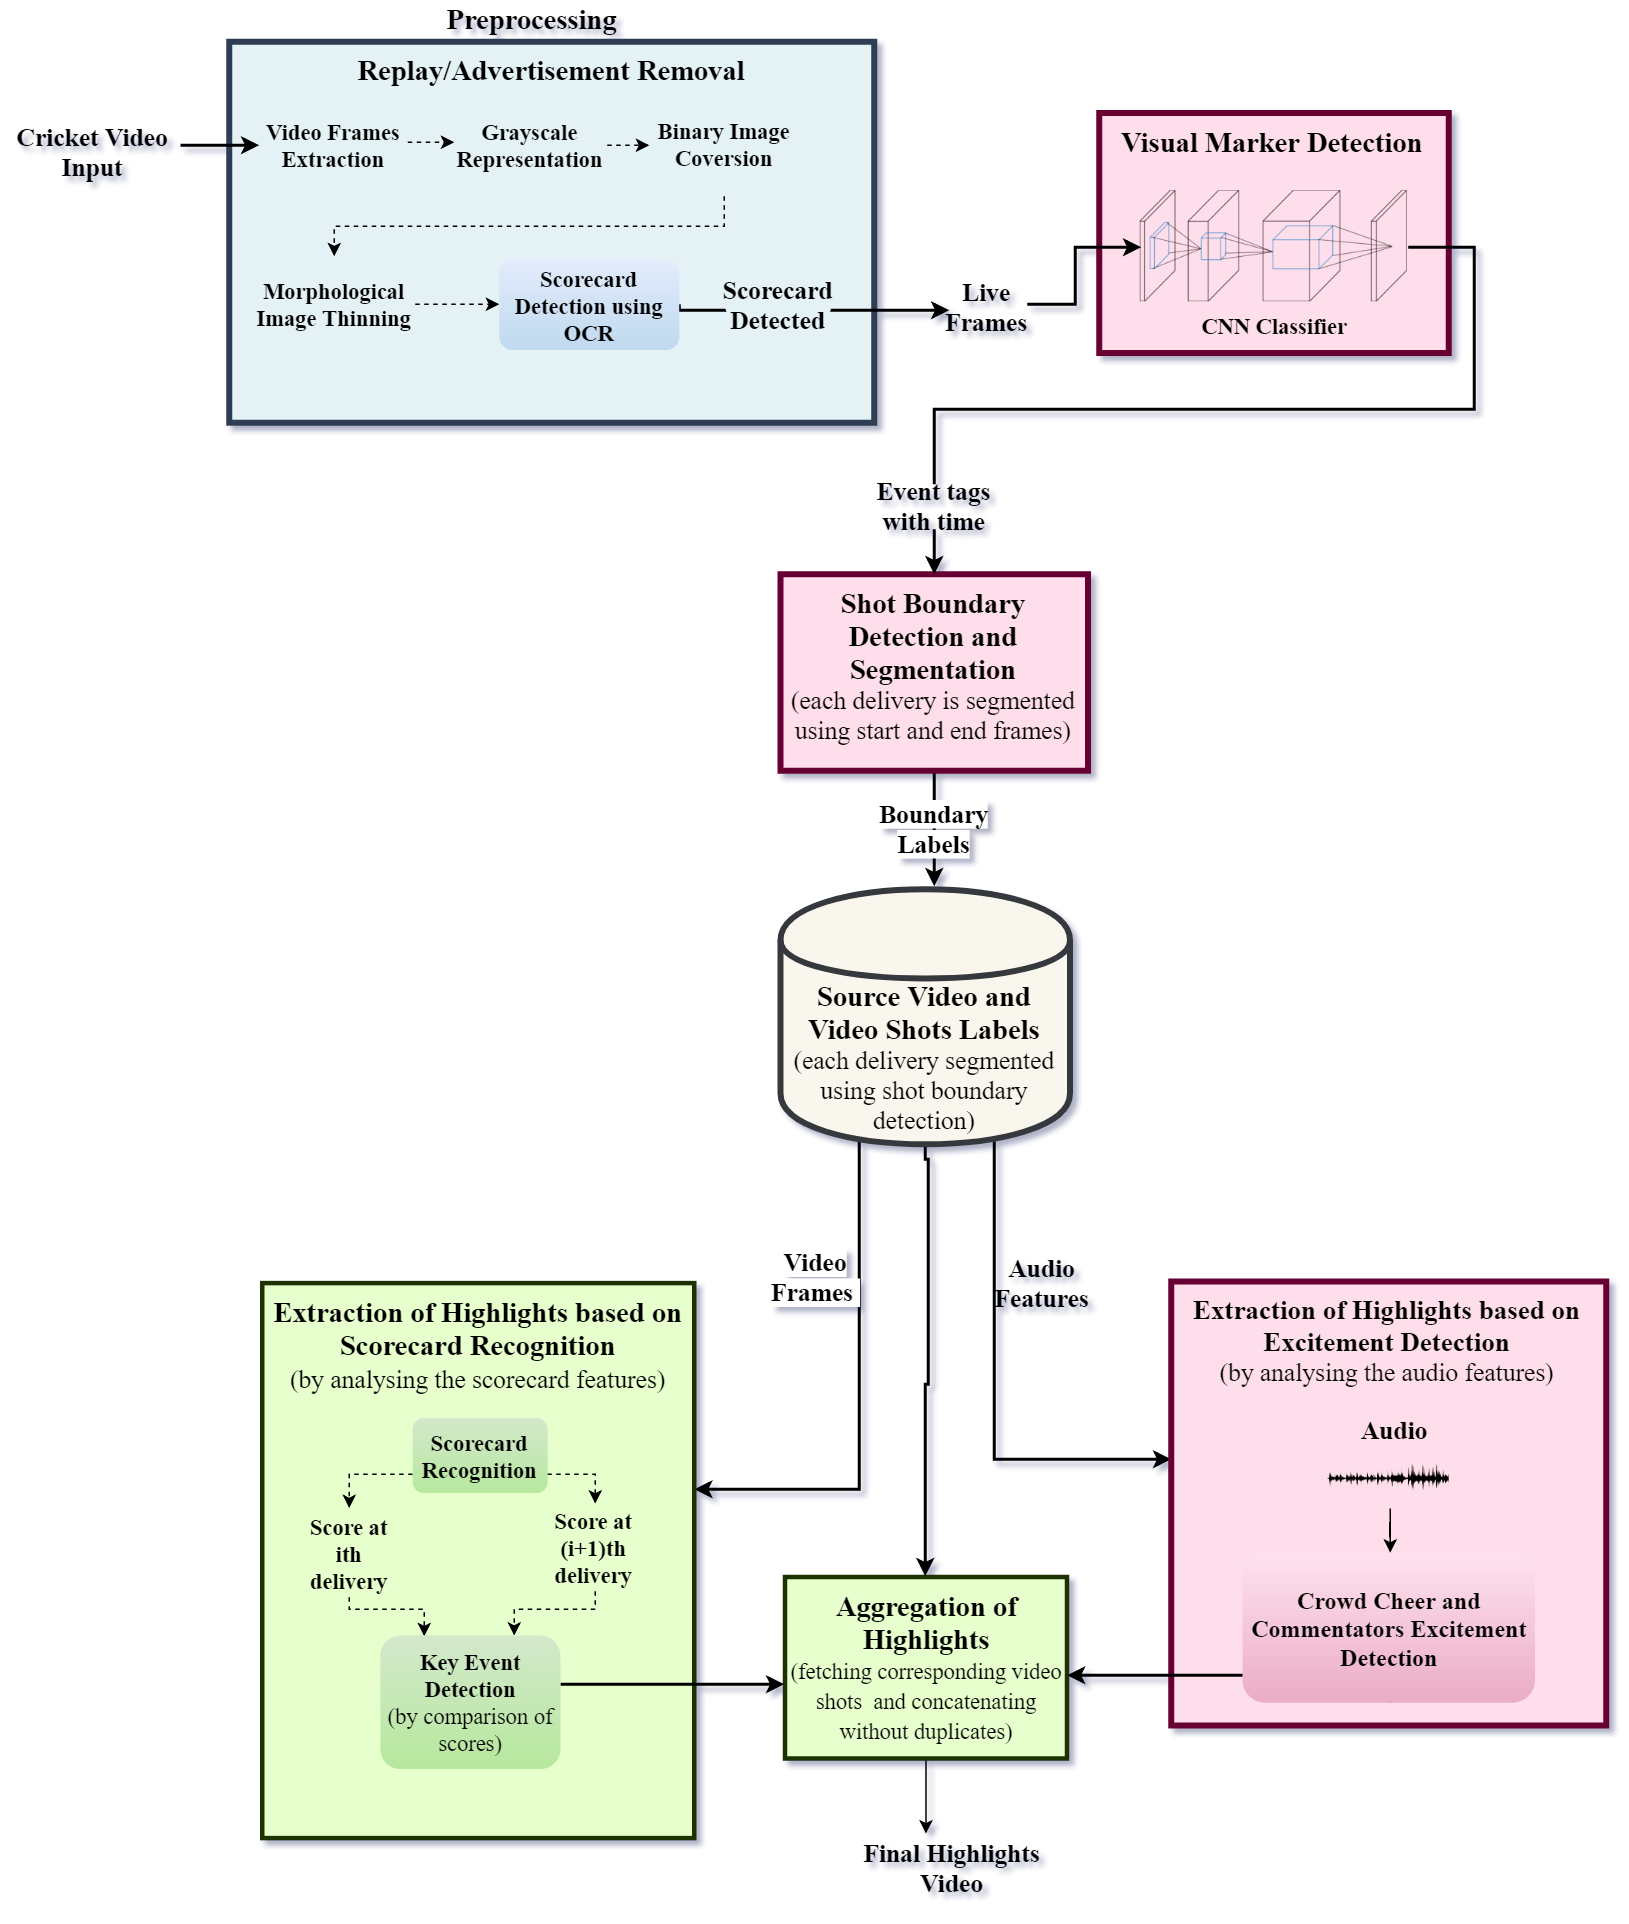
\includegraphics[width=1.0\textwidth,center]{Figures/SysArch.png}
\newpage
\section {Module Design}
\subsection{Preprocessing}
Replays are the repetitive video shots of the key events in the cricket match. Advertisements are unrelated video shots for highlights generation. Therefore, Replays and advertisements are the unwanted shots needed to be removed. This module is used for detection and removal of replays and advertisements by checking the scorecard in the video frames. Absence and presence of the scorecard are used to detect replay and live frames, respectively. Replays and advertisements are categorized as frames without the scorecard. The source video is converted into frames. In order to detect the scorecard by OCR, the frames are converted to gray scale image then to binary image. OCR recognizes the scorecard from the binary image. The frames with the scorecard is live frames which is given to visual marker detection along with their time.
\begin{figure}[h]
    \centering
   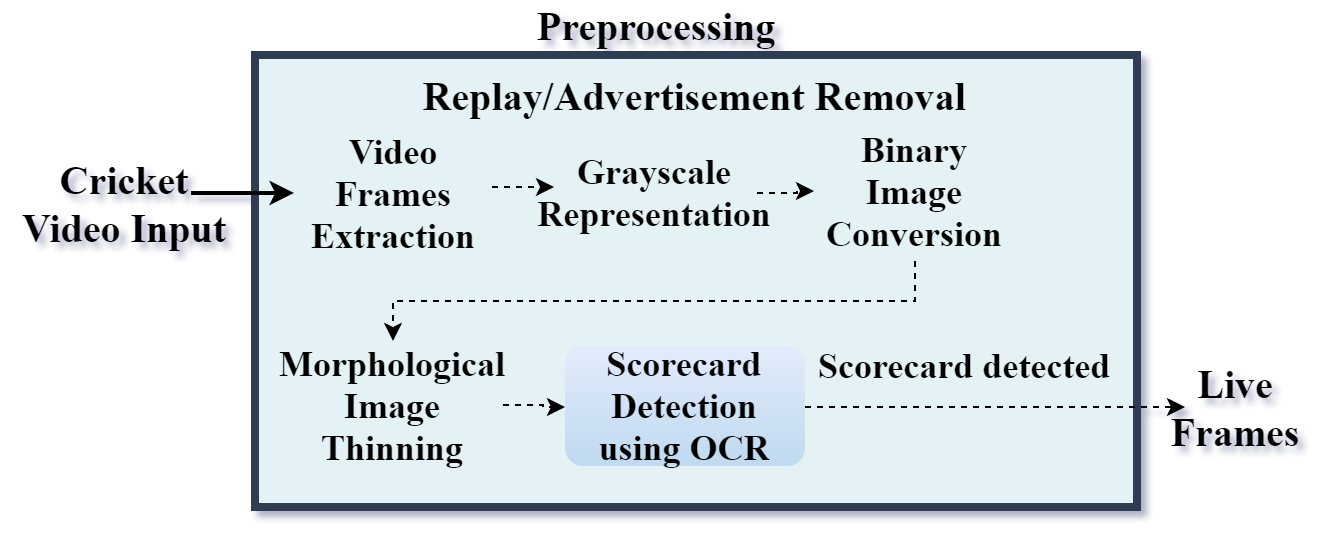
\includegraphics[width=0.25\textwidth,center]{Preprocessing.png}
    \caption{Preprocessing}
    \label{fig:preprocessing}
\end{figure}

\begin{algorithm}
\caption{Preprocessing}
\State \texttt{Input:Source Input Video}\\
\State \texttt{Output:Live Frames}\\
\State \texttt{frames[] := generate\_frames(Source video)}\\
\begin{algorithmic}

\FOR{each frame in frames[]} 
        \State \texttt{image := grayscale(frame)}\\
        \State \texttt{image := binary_conversion(image)}\\
        \State \texttt{text  := OpticalCharacterRecognition(image)}\\
        \IF{is\_scorecard(text):}
                 \State \texttt{mark\_as\_live(frame)}\\
        \ELSE
             \State \texttt{ mark\_as\_replay(frame)}\\
             
        \ENDIF
\ENDFOR
\end{algorithmic}
\end{algorithm}

\newpage
\subsection{Visual Marker Detection}
Events detection is important for shot boundary detection and segmentation. This module is detects events like batting, bowling, crowd, interviews, commentators etc. from the live frames using trained CNN classifier. The CNN is trained for bowling, commentators, interview, field view, crowd, stump view, umpire. The trained model is loaded to predict these classes. The CNN classifier predicts the events for each live frames. The event tag along with the time is given to the shot boundary detection and segmentation.

\begin{figure}[h]
    \centering
   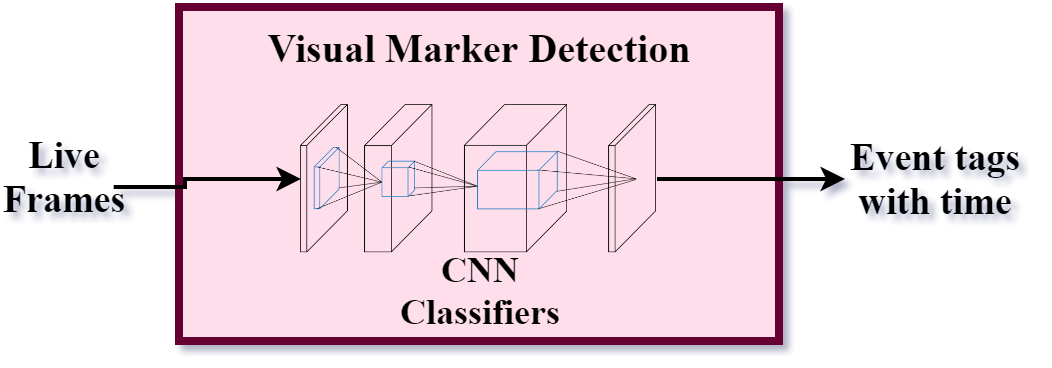
\includegraphics[width=0.25\textwidth,center]{VisualMarkerDetection.png}
    \caption{Visual Marker Detection}
    \label{fig:Visual Marker Detection}
\end{figure}
\begin{algorithm}
\caption{Visual Marker Detection}
\State {Input:Live frames}\\
\State {Output:Event tags with time}\\
\State {model :=load\_trained\_cnn\_classifier()}\\
\begin{algorithmic}
\FOR{\texttt{each frame in frames[]}} 
    \State \texttt{event\_tag :=model.classify(frame)}\\
    \State \texttt{time := fetch\_frame\_time(frame)}\\
    \State \texttt{out\_to\_CSV\_file(event\_tag,time)}\\
\ENDFOR
\end{algorithmic}
\end{algorithm}

\newpage
\subsection{Shot Boundary Detection and Segmentation}
Unwanted events like crowd view, commentators, interviews, etc. are removed. Start/End frames are detected and segmented as video shots. The bowling event is considered as the start of the delivery. Every delivery is till the start of the next delivery. The frames with unwanted events are removed. Using start and end of the delivery, shots are identified. The labels containing start and end time of the delivery is stored for further use.

\begin{figure}[h]
    \centering
   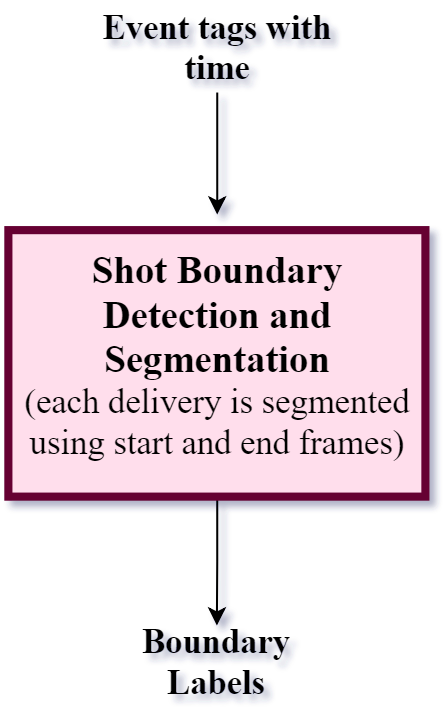
\includegraphics[width=0.25\textwidth,center]{ShotBoundaryDetection.png}
    \caption{Shot Boundary Detection}
    \label{fig:ShotBoundaryDetection}
\end{figure}
\newpage
\begin{algorithm}
\caption{Shot Boundary Detection}
\State \texttt{Input:Event tags}\\
\State \texttt{Output:Segmented delivery labels}\\
\state $i \leftarrow 1$\\
\begin{algorithmic}
\FOR{each event in event[]} 
   \IF{is\_bowling(event)}
                 \State \texttt{start[i] := time(event)}\\
            \State \texttt{ out.write(start)}\\
    \ELSIF{ event in \(commentators, interview, crowd, umpire_signal\)}
             \State \texttt{end[i] := time(event)}\\
             \State \texttt{out.write(end)}\\
        \ENDIF
\ENDFOR
\end{algorithmic}
\end{algorithm}
\newpage
\subsection{Extraction based on Scorecard recognition}

The difference of the score from the first frame of current shot and the first frame of the next shot is checked. If it is 4, 6 then it is added to highlights or if the wicket is increased then it is added to highlights. The score of the start frame of the delivery and the next delivery is recognized. Using the scores, key events are checked. If the score differ by more than 4, it is taken as highlights. If wicket increases, it is also considered as the highlights. Corresponding delivery labels are given as the output to the next module.

\begin{figure}[h]
    \centering
    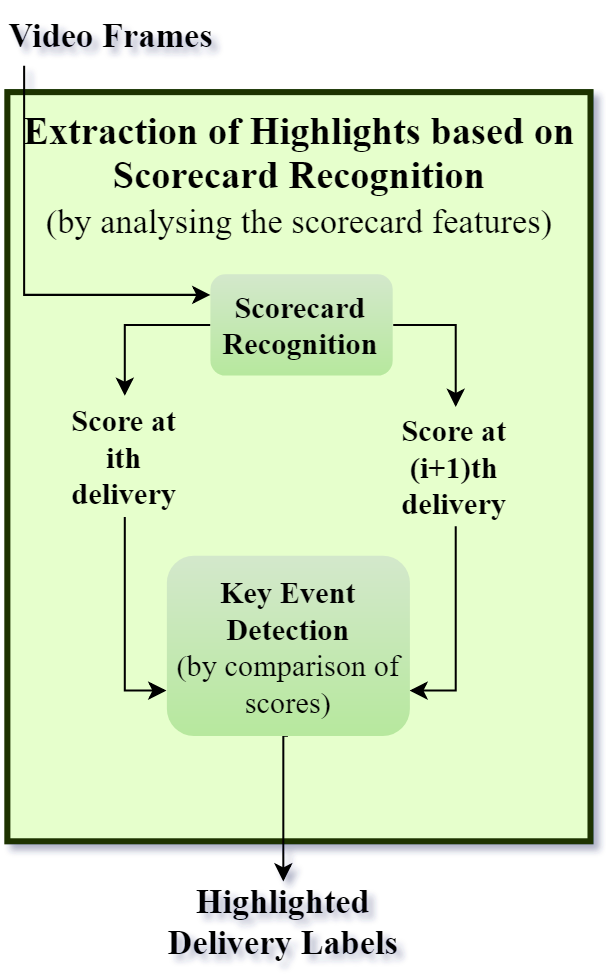
\includegraphics[width=0.25\textwidth]{Scorecard.png}
    \caption{Scorecard recognition}
    \label{fig:Scorecard}
\end{figure}
\begin{algorithm}
\caption{Scorecard recognition}
\State \texttt{Input:video frames of each segmented deliveries}\\
\State \texttt{Output:delivery labels that contains the highlights}\\
\Function{isKeyEvent}{$i$,$highlights$}
\EndFunction
\begin{algorithmic}
\Function{isKeyEvent}{$i$,$highlights$}
\IF{get\_score(get\_frames(i)) - get\_score(get\_frames(i+1)) $>=$4}
          \state{  highlights[i]=1}
\ELSIF{get\_wicket(get\_frames(i)) - get\_wicket(get\_frames(i+1)) $>=$1}
          \state{  highlights[i]=1}
\ELSE \state {highlights[i]=0}
\ENDIF
\EndFunction

\state $i \leftarrow 1$\\
\state highlights[total\_deliveries]\\
\WHILE{$i$ $<$ $total\_deliveries$}
\IF{$isKeyEvent(i,highlights)$}
\ENDIF
\ENDWHILE
\end{algorithmic}
\end{algorithm}
\newpage
\subsection{Extraction based on Excitement Detection}

This module is used for extracting highlights based on excitement using crowd cheer and commentators excitement from audio. The audio energy of the whole is analyzed and computed to get the threshold value then the audio energy of each shots is analyzed and computed, checked with the threshold to identify the highlights. Corresponding labels of the shots are considered as the highlights and given to the next module.

\begin{figure}[h]
    \centering
    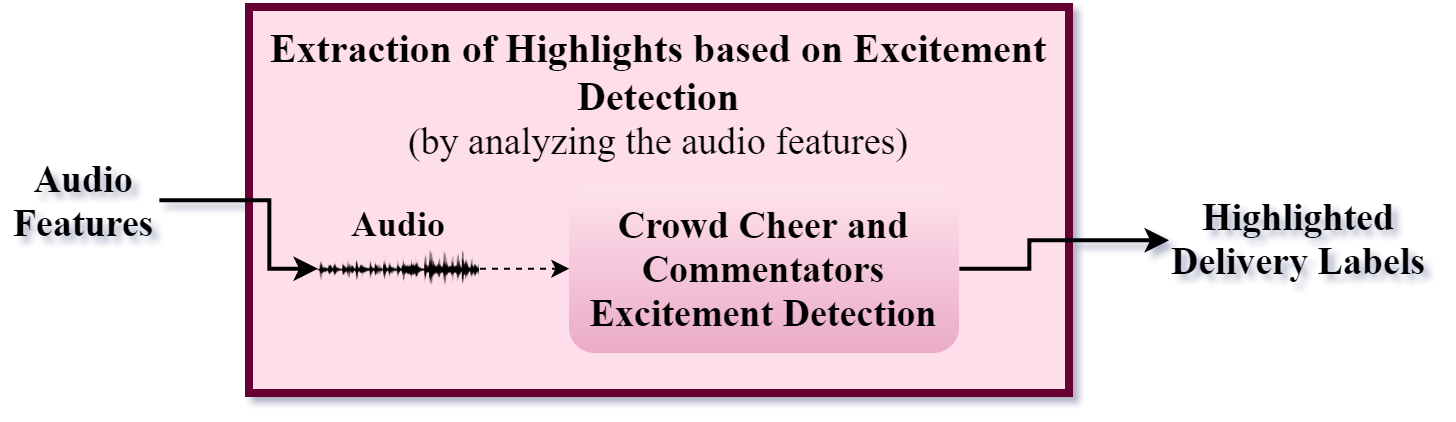
\includegraphics[width=0.25\textwidth]{ExcitementDetection.png}
    \caption{Excitement Detection}
    \label{fig:Excitement}
\end{figure}
\subsection{Aggregation of Highlights}

Highlighted video labels based on scorecard and excitement is combined and corresponding video shots are fetched from the database. These video shots are then concatenated to generate highlights. Highlighted video labels based on scorecard and excitement are combined without duplicates. Corresponding video clips are fetched from the database using the combined labels. These clips are concatenated to form final highlights.
\begin{figure}[h]
    \centering
    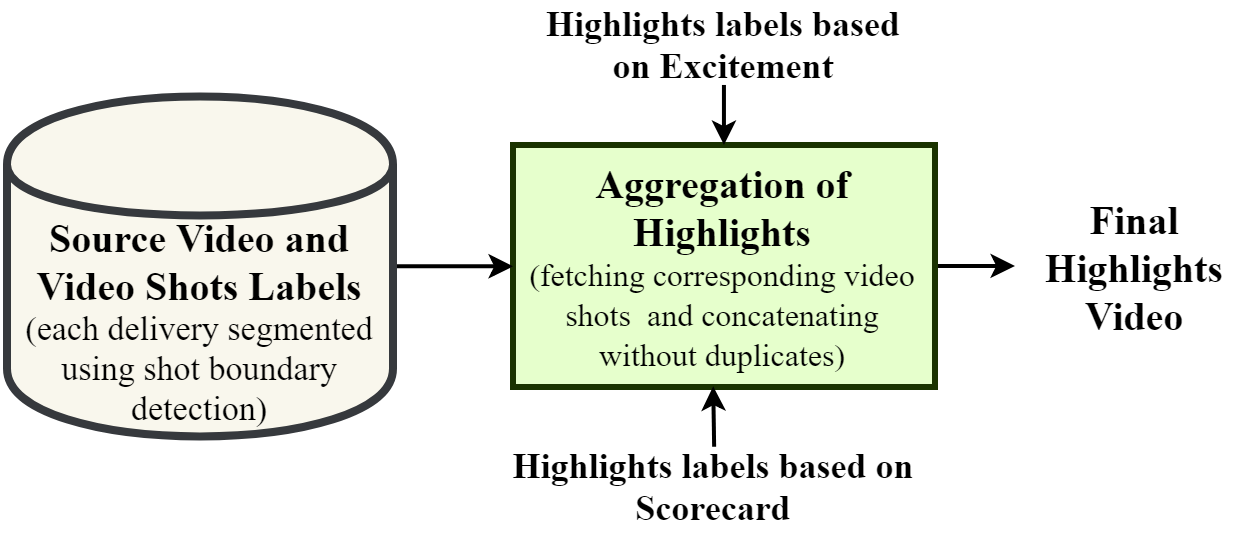
\includegraphics[width=0.25\textwidth]{Aggregation.png}
    \caption{Aggregation of Highlights}
    \label{fig:Aggregation of Highlights}
\end{figure}

\begin{algorithm}
\caption{Aggregation of Highlights}
\begin{algorithmic}
Display(FinalVideo)\\
\begin{table}[ht]
\begin{center}
\begin{tabular}{@{}cc@{}}
Labels1[] & := $HighlightLabels\_scorecard$\\
Labels2[] & := $HighlightLabels\_excitement$ \\
Result[] &:=Label1[] \cup  Label2[]\\
ResultVideo[] &:= FetchVideoFromDatabase(Result[])\\
FinalVideo &:= ConcatenateVideo(ResultVideo)\\
\end{tabular}
\end{center}
\end{table}
\end{algorithmic}
\end{algorithm}
